%----------------------------------------------------------------------------
\chapter{Szöveges PSC leíró nyelv kibővítése}
%----------------------------------------------------------------------------

A nyelvet az \textit{Xtext} technológia segítségével definiáltam.
A nyelv két új elemmel bővült:

\begin{itemize}
    \item időzített feltétel
    \item óraváltozó nullázása
\end{itemize}

\begin{figure}[!ht]
    \centering
    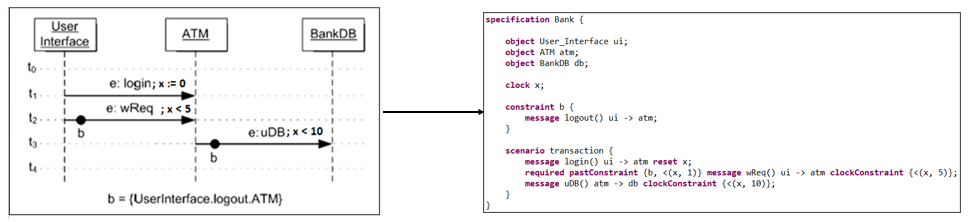
\includegraphics[width=150mm, keepaspectratio]{figures/11abra.png}
    \caption{\textit{TPSC} diagramból szöveges leírás az \textit{Xtext} nyelv használatával.}
    \label{xtext_language_example}
\end{figure}

A \ref{xtext_language_example} ábrán látható, hogy egy \textit{TPSC} diagramot hogyan tudunk leírni a nyelvünk segítségével.
Definiálhatjuk a diagramban szereplő objektumokat, a megkötéseket amiket használni fogunk és végül, hogy milyen üzenetek vannak a követelményünkben.

\begin{figure}[!ht]
    \centering
    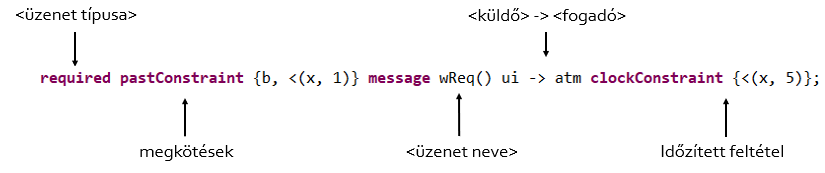
\includegraphics[width=150mm, keepaspectratio]{figures/12abra.png}
    \caption{Egy \textit{TPSC} üzenet felépítése a definiált \textit{Xtext} nyelvben.}
    \label{xtext_message}
\end{figure}

A \ref{xtext_message} ábrán látszik, hogy megjelenik a \textit{clockConstraint} kulcsszó ami egy időzítési feltétel megadására szolgál.
A kulcsszó után kapcsos zárójelek közt megadható a feltétel.
A \textit{reset} kulcsszó az óraváltozó nullázására szolgál.